\documentclass{llncs}

%%%%%%%%%%%%%%%%%%%%%%%%%%%%%%%%%%%%%%%%%%%%%%
\usepackage[utf8]{inputenc}%                 %
\usepackage[T1]{fontenc}%                    %
\usepackage{lmodern}%                        %
\usepackage{graphicx}%                        %
                                             %
\usepackage{xcolor}%                         %
\newcommand{\gnramos}[1]{\textcolor{red}{#1}}%
%%%%%%%%%%%%%%%%%%%%%%%%%%%%%%%%%%%%%%%%%%%%%%

\begin{document}%
\title{XXXXX analysis of high school girls' perspective of the in Brazil's Distrito Federal}%
%
\author{Roberto Mourão\inst{1}%
\and Guilherme N. Ramos%
\and Maristela}%
%
\institute{University of Brasília, Brasília - DF, Brazil,\\
\email{mholanda@unb.br},\\%
WWW home page: \texttt{http://cic.unb.br}}%

\maketitle%

\begin{abstract}%
% The abstract should summarize the contents of the paper
% using at least 70 and at most 150 words. It will be set in 9-point
% font size and be inset 1.0 cm from the right and left margins.
% There will be two blank lines before and after the Abstract. \dots
Nos últimos anos, vem sendo realizadas reflexões sobre as razões da baixa entrada feminina nos cursos de graduação na área da Computação. Para entender esse processo no âmbito do Distrito Federal no Brasil, durante 5 anos um grupo de docentes do Departamento de Ciência da Computação da Universidade de Brasília coletou dados sobre a percepção das alunas do ensino médio. Neste artigo é apresentado uma análise XXXX dos dados coletados.%

\keywords{computer science,gender}%
\end{abstract}%

\section{Introduction}\label{sec:intro}%

%Begin Maristela
In Brazil, the choice of an undergraduate major in the area of Computer Sciences is not among the top choices for girls in high school when contemplating a career. As \cite{maia_2016} presents, between 2000 and 2013 in Brazil, an average of only 17\% of all graduates in various Computer Science majors were women. This research covered majors in Computer Science, Computer Engineering, and Information Systems, among others. Particularly, in the Federal District, at the University of Brasilia, which currently has approximately 30,000 students enrolled in undergraduate programs, the reality is even worse, where in the past 10 years, according to \cite{couto_2014} only 10\% were women.

	Responding to the low incidence of women in Computer Science majors, recently researchers have given much thought about how to improve this scenario and proposed strategies to encourage girls to pursue a profession in the Computer Sciences   \cite{cohoon_2002} \cite{couto_2014}  \cite{gurer_2002}  \cite{maia_2016}. Brazil and other countries have developed initiatives to debate this issue. Specifically, the Institute of Electrical and Electronics Engineers (IEEE) has a program which address the problem: the IEEE Women in Engineering (WIE) \cite{wie2017}. The WIE is a major professional and international organization dedicated to promoting women scientists and engineers. Another prominent program in promoting women in the area of Computers is ?Girls who Code? \cite{girlsWC_2017}, which has over 40,000 members and various initiatives to increase the participation of girls in Computer Sciences over various regions in the United States. Another initiative from the United States is the ?Grace Hopper Celebration of Women in Computer Sciences? event, which is the biggest event worldwide for discussing the theme of women in the field. In 2016 alone 15,000 people from 87 countries participated in the 700 presentations \cite{GHC_2017}.

	In Brazil, since 2007, the Brazilian Society of Computing Conference held the Women in Information and Technology Workshop (WIT), to discuss the theme. Brazilian governmental agencies, such as the Ministry of Science and Technology released calls for submissions of research projects specifically related to the education of girls in Computing or Physical Science majors \cite{cnpq_2017}. Aiming to gather information about the perceptions of high school girls regarding computer science, the Department of Computer Science at the University of Brasilia, developed the project, Meninas.comp: computação  tambem e coisa de menina, Girls.comp: computer science is a girl thing too.

%End Maristela

\gnramos{Falar da análise realizada (Roberto e Guilherme)}%

Between the years of 2012 and 2014, we contacted thousands of girls in Middle and High School to investigate the relationship between their intention to apply for an undergraduate course in Computer Science and their affinity with the field and computing tools. We used the Apriori algorithm on the collected data, searching for interesting association rules and insights on the girls' interest in CS and their background.

This following sections of this work are organized as follows: Section~\ref{sec:background} presents related work and background information on this approach, Section~\ref{sec:mining} describes details of the data mining applied, Section~\ref{sec:results} provides our experimental results and our finds and Section~\ref{sec:conclusion} presents concluding remarks.
%
\section{Related Works}\label{sec:related}%
There have been several studies addressing the gender issue in Computer Science. Lagesen describes CS as STEM field that has excluded women~\cite{vivian_2007}. Putnik et al. presents data from Yugoslavia, comparing gender ratios and observing a higher number of men compared women~\cite{zoran_2017}.

Stout et al. in~\cite{jane_2016} and Cheryan et al. in~\cite{sappa_2013} provide studies about stereotyping in Computer majors, also arguing that there is a higher ratio of men than women in this field in the US. Likewise, Mercier et al. present surveys, drawings, and interviews which were used to examine the perception of US middle school students about characteristics of knowledgeable computer users~\cite{Mercier_2006}. These results showed cultural stereotypes of a computer user: 89\% were male and 94\% wore glasses.

Keinan et al. show data that the ratio of graduated women from Bachelor's programs in CS was of almost 40\% in 1984, dwindling to 20\% by 2006 in the US~\cite{keinan_2017}. Vardi has similar results, and adds that in 2013 and 2014, only 14.7\% of those graduates were women~\cite{moshe_2015}.

Papastergiou used descriptive statistics, principal component analysis and analysis of variance in~\cite{papastergiou_are_2008} to investigate 358 Greek high school students' intentions and motivation for pursuing academic studies in CS. This study looked into several factors, such as the influence of family and academic environment on their career choices, their perception of a professional career in CS, and their self-efficacy beliefs regarding computers. The analysis showed that a lack of exposure to and use of a computer at home and in school from early stages in the students' lives seems to be the main factor in discouraging them from studying CS, specially considering the data for girls.

Anderson et al. applied means, \mbox{Mann-Whitney} $U$ test comparison, and non-parametric statistics in~\cite{anderson_because_2008} to study possible factors related to low rates of female participation in education pathways leading to information and communications technology (ICT) professions, considering data from a three-year period. The survey had binary options, such as ``I am very interested in computers'' and ``I am not interested in computers'', was presented to 1,453 high school girls in their Senior year. The study identified two factors associated with a woman's aversion to ICT careers: the perception that the subject is boring, and an intense dislike of computers.

Maia describes a similar situation in~\cite{maia_2016}, presenting a study on female participation in university majors in CS in Brazil, based on the Higher Education Census data from the Ministry of Culture and Education between the years of 2000 and 2013. One of the issues raised was that while the number of male graduates increased 98\% in the period, that of female graduates decreased 8\%.

The Department of Computer Science\footnote{\url{http://cic.unb.br}} at the University of Brasília (UnB) currently offers three undergraduate degrees related to CS: Bachelor of Computer Science (since 1987), Licentiate in Computing (since 1997), and Computer Engineer (since 2008). Figure~\ref{fig:computerMajorUnB} shows gender data for students enrolled in them.

\begin{figure}%
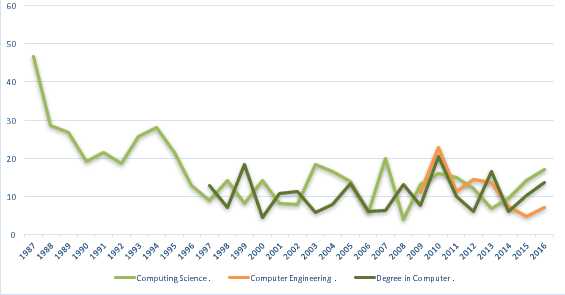
\includegraphics[width=\textwidth]{img/Figure1-girlsUnB}%
\caption{Ratio of female students enrolled in UnB's CS majors.}%
\label{fig:computerMajorUnB}%
\end{figure}%

In 1987, when the Bachelor course began, the gender difference between students enrolled was relatively low: 47\% of were female. However, this number decreased over time and, in 1997, this percentage fell to 10\%; by 2013 it was only 6\%. The Licentiate degree's ratio oscillates roughly around 11\%, while the Computer Engineer, which already began with low numbers, saw them fall to less than 12\% in the past three years.

We can see from the data that the difference between the number of male and female students enrolled in a CS major at UnB has decreased over the years, similar to what was reported in the before mentioned surveys. Given this alarming decline, and the widening disparity between male and female representations in the field of Computer Science, our work aims to investigate possible reasons for such scenario.\gnramos{Acho que poderia ficar explícito o porque da necessidade de mais mulheres. (``o que a diversidade acrescenta?'' e o que poderia ser feito com os resultados para melhorar a situação)}
%
\section{Data Mining}\label{sec:mining}%
%3. Teoria sobre a análise dos Dados (Roberto e Guilherme).%

Data mining is the process of discovering insightful patterns and predictive models from data~\cite{Zaki2014}, trying to make sense of usually large amounts of information in some domain~\cite{Cios2007}. \gnramos{In this work, the primary interest is the gender gap in the fields of the "hard sciences," so we attempt to understand the profiles of women intending to enroll in undergraduate studies, especially those interested in Computer Science.}

From 2012 to 2014, 1709 people were polled, responding a questionnaire\footnote{\url{https://github.com/rnmourao/women\_computer\_science/blob/master/data/questionnaire.pdf}}. The idea was to obtain information on their perceptions of their future undergraduate studies.

\subsection{Poll}\label{sec:mining:poll}%
The poll had 18 questions, decribed below:

\begin{enumerate}
    \item Gender:
        \begin{enumerate}
            \item Female
            \item Male
        \end{enumerate}
    \item Educational Stage:
        \begin{enumerate}
            \item Middle School
            \item High School (10th Grade)
            \item High School (11th Grade)
            \item High School (12th Grade)    
            \item Adult Education Program
            \item College        
        \end{enumerate}
    \item Which is your Field of Interest?
        \begin{itemize}
            \item Biology-Health Sciences 
            \item Human Sciences
            \item Exact Sciences    
        \end{itemize}
    \item Are you intend to apply for a Computer Science course?
        \begin{itemize}
            \item Yes
            \item No
            \item Maybe
        \end{itemize}
    \item Mark all places where you use computers:
        \begin{itemize}
            \item Home
            \item Relatives' House
            \item Friends's House
            \item School
            \item Work
            \item Lan House
            \item Library
            \item Digital Inclusion Centre
        \end{itemize}
    \item Mark all softwares or activities you use or do with  a computer:
        \begin{itemize}
            \item Text Editor (Microsoft Word, etc.)
            \item Image Editor
            \item Spreadsheet
            \item Database
            \item Web Browser (Search Engines, News, etc.)
            \item Social Networks (Facebook, Orkut, etc.)
            \item E-mail
            \item Games
            \item Create Web Pages
            \item Create Softwares
            \item Other Softwares
        \end{itemize}
    \item Does a Computer Science course only teaches how to use software?
        \begin{itemize}
            \item Yes
            \item No
            \item Maybe
        \end{itemize}
    \item Does a Computer Science course uses easy Math?
        \begin{itemize}
            \item Yes
            \item No
            \item Maybe
        \end{itemize}    
    \item Does the majority of Computer Science's students are male?
        \begin{itemize}
            \item Yes
            \item No
            \item Maybe
        \end{itemize}
    \item Is it necessary to know how to use computers to apply for a Computer Science course?
        \begin{itemize}
            \item Yes
            \item No
            \item Maybe
        \end{itemize}                            
    \item Is it necessary to graduate in Computer Science to work in the area?
        \begin{itemize}
            \item Yes
            \item No
            \item Maybe
        \end{itemize}        
    \item Would your family like you to apply for a Computer Science course?
        \begin{itemize}
            \item Yes
            \item No
            \item Maybe
        \end{itemize}                
    \item It is difficult to get a job after undergraduate in Computer Science?
        \begin{itemize}
            \item Yes
            \item No
            \item Maybe
        \end{itemize}        
    \item Who works with Computer Science has few hours of leisure?
        \begin{itemize}
            \item Yes
            \item No
            \item Maybe
        \end{itemize}    
    \item Does working with Computer Science allow you to exercise creativity?
        \begin{itemize}
            \item Yes
            \item No
            \item Maybe
        \end{itemize}
    \item Does working with Computer Science brings prestige?
        \begin{itemize}
            \item Yes
            \item No
            \item Maybe
        \end{itemize}    
    \item Does working with Computer Science allow you to earn a good salary?
        \begin{itemize}
            \item Yes
            \item No
            \item Maybe
        \end{itemize}
    \item Does working with Computer Science allow you to work in other fields?
        \begin{itemize}
            \item Yes
            \item No
            \item Maybe
        \end{itemize}                                    
\end{enumerate}

The questions were translated into 36 variables, as following: Gender, Educational.Stage, Field.Interest, Interest.CS, Computer.Home, Computer.Relatives, Computer.Friends, Computer.School, Computer.Work, Computer.Lan.House, Computer.Library, Computer.Digital.Inclusion.Centre, Use.Text.Editor, Use.Image.Editor, Use.Spreadsheet, Use.Database, Use.Internet, Use.Social.Network, Use.Email, Use.Games, Create.Web.Pages, Create.Softwares, Use.Other.Softwares, Only.Teaches.Software, Has.Low.Math, Man.Majority, Need.Know.Computer, Need.Higher.Education, Family.Approval, Low.Employability, Low.Leisure, Use.Creativity, Bring.Prestige, Good.Salary, Interdisciplinarity, and Year.

\gnramos{descrição das perguntas, motivações, tipos de respostas (categoricas, numericas...)}

\subsection{Statistical Analysis}\label{sec:mining:stat}%
The usual pre-processing tasks were quickly done; all questionnaires were created and processed by CESPE\footnote{\url{http://www.cespe.unb.br/}}, a specialized research center, and the results given in simple spreadsheets. The data for all years was consolidated in a single spreadsheet\footnote{\url{https://github.com/rnmourao/women\_computer\_science/blob/master/data/raw.xlsx}}, which was then processed in the \texttt{R} programming language.

The script cleans up the data (empty columns, whitespaces, etc.) and begins to process it for analysis. The first step is to consider only the data for the 1709 female respondents. The data is distributed throughout the years as illustrated in Figure~\ref{fig:RespondentsPerYear}. \gnramos{Descrição desta informação}.

\begin{figure}[h!]%
\includegraphics[width=\textwidth]{img/RespondentsPerYear}%
\caption{Number of respondents per year.}%
\label{fig:RespondentsPerYear}%
\end{figure}%

Figure~\ref{fig:EducationalStage} shows how the respondents were distributed by educational stage, indicates that \gnramos{qual a relevância desta informação?},

\begin{figure}[h!]%
\includegraphics[width=\textwidth]{img/EducationalStage}%
\caption{Educational Stages of respondents.}%
\label{fig:EducationalStage}%
\end{figure}%

Figure~\ref{fig:FieldOfInterest} shows the respondents' interest in different fields of study. These results indicate that, throughout the years, the percentages for each choice remains more or less the same with an average of $41\%$ for \emph{Biology-Health Sciences}, $22\%$ for \emph{Exact Sciences} and $33\%$ for \emph{Human Sciences}.

\begin{figure}[h!]%
\includegraphics[width=\textwidth]{img/FieldOfInterest}%
\caption{Respondents' fields of interest.}%
\label{fig:FieldOfInterest}%
\end{figure}%

Figure~\ref{fig:InterestInCS.pdf} shows the respondents' interest in applying for a Computer Science course. This results indicate that $31\%$  \emph{have interest}, $28\%$  \emph{have no interest}, and $41\%$  \emph{have doubt}

\begin{figure}[h!]%
\includegraphics[width=\textwidth]{img/InterestInCS.pdf}%
\caption{Respondents interested in Computer Science.}%
\label{fig:InterestInCS.pdf}%
\end{figure}%

% APRIORI %%%%%%%%%%%
As described earlier, the data consisted of a group of 1,709 questionnaires with 18 questions each. There were 3,707 surveys, but some were excluded for many reasons: some were answered by men, others were answered by College or Adult Education Program students. None of these were adequate for the study. The questionnaires from 2011 were excluded because the poll was conducted differently of the others years.

An Apriori's association rule mining algorithm was performed on the data, with the minimum confidence level equal to 50\%, and with a maximum number of 3 items in an itemset. A filter was applied to select only the rules involving the variable \emph{CS.Interest} on the rules' right-hand sides. The rules were analyzed considering support, confidence and lift metrics.
%
\section{Experimental Results}\label{sec:results}%

% Family.Approval, Use.Creativity %

The association rule mining resulted in 10 rules involving the students' interest in Computer Science. Figure \ref{fig:apriori} shows rules' left-hand side (lhs), rules' right-hand side (rhs), support, confidence and lift metrics.

\begin{figure}%
\includegraphics[width=\textwidth]{img/apriori.pdf}%
\caption{Rules with higher confidence, ordered by lift.}%
\label{fig:apriori}%
\end{figure}%

The rules found had very close levels of confidence, between 0.56 and 0.59. The lift metric was similar, with values between 1.8 and 1.9. Figure \ref{fig:plot.apriori} shows in a chart this conclusions.

\begin{figure}%
\includegraphics[width=\textwidth]{img/{plot.apriori}.pdf}%
\caption{Rules with higher confidence, ordered by lift.}%
\label{fig:plot.apriori}%
\end{figure}%

% Family.Approval %
A general result was the presence of \emph{Family.Approval=Yes} item in all rules. The values found in \emph{Family.Approval} attribute were three: \emph{Yes}, indicating the student believes that her family may approve her application for a Computer Science course; \emph{No}, stating that the student believes in family disapproval; and  \emph{Maybe} indicates that the students have doubts about her family's opinion. Figure \ref{fig:plot.Family.Approval} shows the number of respondents by answer involving \emph{Family.Approval} and \emph{CS.Interest} attributes.

Support metrics found in Figure \ref{fig:apriori} are varying from 10 to 12\%. This percentage is significant when compared to the total of respondents interested in CS (31\%).

% Confidence varied from 50 to 59\%. %

% Lift varies from 1.8 to 1.9. This metric %


The first rule on figure \ref{fig:apriori} had the highest confidence level. The confidence metric, in this case,  states that 59\% of times a respondent believes that has family's approval and doesn't use computer at home, then she will have an interest in CS. The 1.9 lift indicates that there are 90\% of chance that the family's approval, the lack of use of computer at home and the interest to apply for a CS course are correlated. 

The second rule on figure \ref{fig:apriori} states that 58\% of times a respondent believes that has family's approval and believes that CS uses creativity, then she will have an interest in CS. The 1.9 lift indicates that there are 90\% of chance that the family's approval, the perception of creativity in CS and the interest to apply for a CS course are correlated.

The third rule 

The second rule in figure \ref{fig:apriori} indicates that family's approval is, per si, an important rule. Confidence and lift are only a bit smaller than their first rule pairs. The figure \ref{fig:plot.Family.Approval} has the number of respondents per girl's guess of family's opinion and own answer about interest in CS.

\begin{figure}%
\includegraphics[width=\textwidth]{img/{plot.Family.Approval}.pdf}%
\caption{Amount of respondents by answer in Family.Approval and in CS.Interest.}%
\label{fig:plot.Family.Approval}%
\end{figure}%

While the \emph{Family.Approval} attribute appears as an isolated rule in figure \ref{fig:apriori}, it is noticeable that this does not happen for \emph{Use.Creativity}. The absence of such rule indicates that creativity alone is not a strong stimulus to respondents decide for Computer Science. Figure \ref{fig:plot.Use.Creativity} shows the number of respondents per girl's opinion about the use of creativity in CS and the interest in applying for a Computer Science course.

\begin{figure}%
\includegraphics[width=\textwidth]{img/{plot.Use.Creativity}.pdf}%
\caption{Amount of respondents by answer in Use.Creativity and in CS.Interest.}%
\label{fig:plot.Use.Creativity}%
\end{figure}%%
\section{Conclusion}\label{sec:conclusion}%

In recent years, the area of Computer Science has had the participation of few women in the profession, showing that girls have not shown interest in majoring or becoming professionals in this field. Given this scenario, research aimed at understanding their motives for not choosing a major or career in computers is important to promoting actions that will reduce the disparity between boys and girls entering the field, by increasing participation of the girls.

Data mining was performed in the answers from a questionnaire applied from 2011 to 2014, and the Apriori algorithm showed that the single most important factor for a Middle or High School girl deciding whether to pursue a degree in a CS major is her family's approval of this choice. This result provides insights to guide further actions to reduce the gender gap in the field.

Future works include: improving the questionnaire; applying the analysis to data for  Middle and High School boys, for comparison, as well as to students who have enrolled in a CS major; and investigating other data mining approaches for knowledge discovery.
%

\bibliographystyle{splncs03}%
\bibliography{bibliography}%
\end{document}%
